\chapter{Material and Methods}
\label{chp:material_methods}
% ---------------------------------------------------------------------------------------------------

% ===================================================================================================
\section{Regression and interpolation methods}
% ===================================================================================================

\begin{itemize}
\itemsep0em
  \item explain the work done on regression and interpolation
  \item explain their relation with emulation
  \item explian extrapolation, when it can be done and how reliable it can be
\end{itemize}


% ===================================================================================================
\section{Development of \textit{FullSWOF\_2D} interaction tools}
% ===================================================================================================

\begin{itemize}
\itemsep0em
  \item explain the work done
  \item list the functions developed and their function
  \item mention \textit{fswof2d} repository
  \item explain how to install the package?? \noteseb{does this make sense here?? should go in the README}
\end{itemize}

As already mentioned in section \colseb{mention which section} \textit{FullSWOF\_2D-v1.07.00} was chosen as \emph{overland flow simulator} in order to generate the required datasets.
\textit{FullSWOF\_2D} needs at least three input files in order to run simulations:

\begin{itemize}
\itemsep0em
  \item \textit{topography}: a text file specifying the topography of the domain
  \item \textit{parameters}: a text file specifying the values set for the simulation parameters
  \item \textit{huv\_init}: a text file defining the initial conditions of the problem (initial water height and initial water velocity at every point of the grid)
\end{itemize}

In order to generate these files, interaction functions were developed with the open source tool \textit{Octave 4.2.1} \autocite{octave_community_gnu_2018}.
The interaction functions were grouped into the Octave package \textit{fswof2d} available at \url{https://bitbucket.org/binello7/fswof2d}.\\

The package includes the following functions, all of which are distributed under \textit {GPLv3} license \autocite{smith_quick_2014}.

\begin{itemize}
\itemsep0em
  \item center2node.m
  \item csec\_channel2lvlsym.m
  \item dataconvert.m
  \item extrude\_csec.m
  \item huv2file.m
  \item matplotlib\_cm.m
  \item node2center.m
  \item params2file.m
  \item read\_params.m
  \item topo2file.m
\end{itemize}

% ---------------------------------------------------------------------------------------------------
\subsection*{center2node.m}
% ---------------------------------------------------------------------------------------------------
\textit{function x = center2node (cx, x0)}\\



% ---------------------------------------------------------------------------------------------------
\subsection*{node2center.m}
% ---------------------------------------------------------------------------------------------------
\textit{function cx = node2center (x)}\\

\textit{FullSWOF\_2D} uses a regular uniform grid in order to solve the \emph{shallow water equation} with the finite volume method (FVM).
The equations are solved at the center of every cell.
After creating the vector defining the grid nodes, one can use the \textit{center2node} function to compute the centers of the grid cells.
This is particularly useful because the $(x,y)$ coordinates saved to the \textit{topography} file have to be the coordinates of the cell centers.
A short usage example would be:

\begin{lstlisting}
  # define the domain length in x-direction
  Lx = 100;
  # define the number of nodes
  Nx = 200;
  # create nodes of the regular grid in x-direction
  xn = linspace (0, Lx, Nx);
  # create vector of cell centers
  xc = node2cdenter (xn);
\end{lstlisting}



% ===================================================================================================
\section{Didactic example: emulator \noteseb{appropriate to use emulator here? other suggestions?} of " the weir equation"}
% ===================================================================================================

\begin{itemize}
\itemsep0em
  \item present it as a didactic example
  \item use it to compare GP (prior knowledge) with e.g. deep neural networks: how many points can we have?
  \item mention grid convergence study (results go in the appendix A)
  \item mention problem with FullSWOF boundary conditions
  \item define well results and methodology
\end{itemize}

% ---------------------------------------------------------------------------------------------------
\subsection{Methodology}
% ---------------------------------------------------------------------------------------------------

Short methodology of how the mechanistic emulator of the weir equation was developed, without subdivision into further subsections.


% ---------------------------------------------------------------------------------------------------
\subsection{Results and discussion}
% ---------------------------------------------------------------------------------------------------

Present and discuss briefly the results of this toy emulator.


% ===================================================================================================
\section{Generating the synthetic topography}
% ===================================================================================================

In order to run the simulations necessary for building the \textit{emulator}, a synthetic topography was produced.
The synthetic topography, in comparison with a real one, has the advantage of having a much smoother surface.
This ensures convergence of the solution at lower grid resolution, reducing therefore the simulation runtime.
The procedure to follow in order to build the \textit{emulator} with a real topography would be exactly the same.\\

The synthetic topography was produced using the software \textit{Octave 4.2.1} \noteseb{how to cite this?} \autocite{octave_community_gnu_2018} and the developed package \textit{fswof2d} \noteseb{cite it? how?} in order to export it to a format compatible with \textit{FullSWOF\_2D-v.1.07.00} \autocite{delestre_fullswof:_2014} \noteseb{put the citation every time that it is mentioned?}.
The generated topography is visible in Fig.~\ref{fig:topography}.
It represents a catchment of $\SI{2}{\kilo\meter} \times \SI{2}{\kilo\meter}$ composed of a sloping plane with three Gaussian bumps on the top.
The Gaussian bumps have different heights and widths and generate a \emph{Y-shaped channel} which extends from the upper and left boundary down to the lower boundary.
A paraboloid was added to the plane to promote the accumulation of water in the channel.\\


\begin{figure}[htpb]
  \centering
  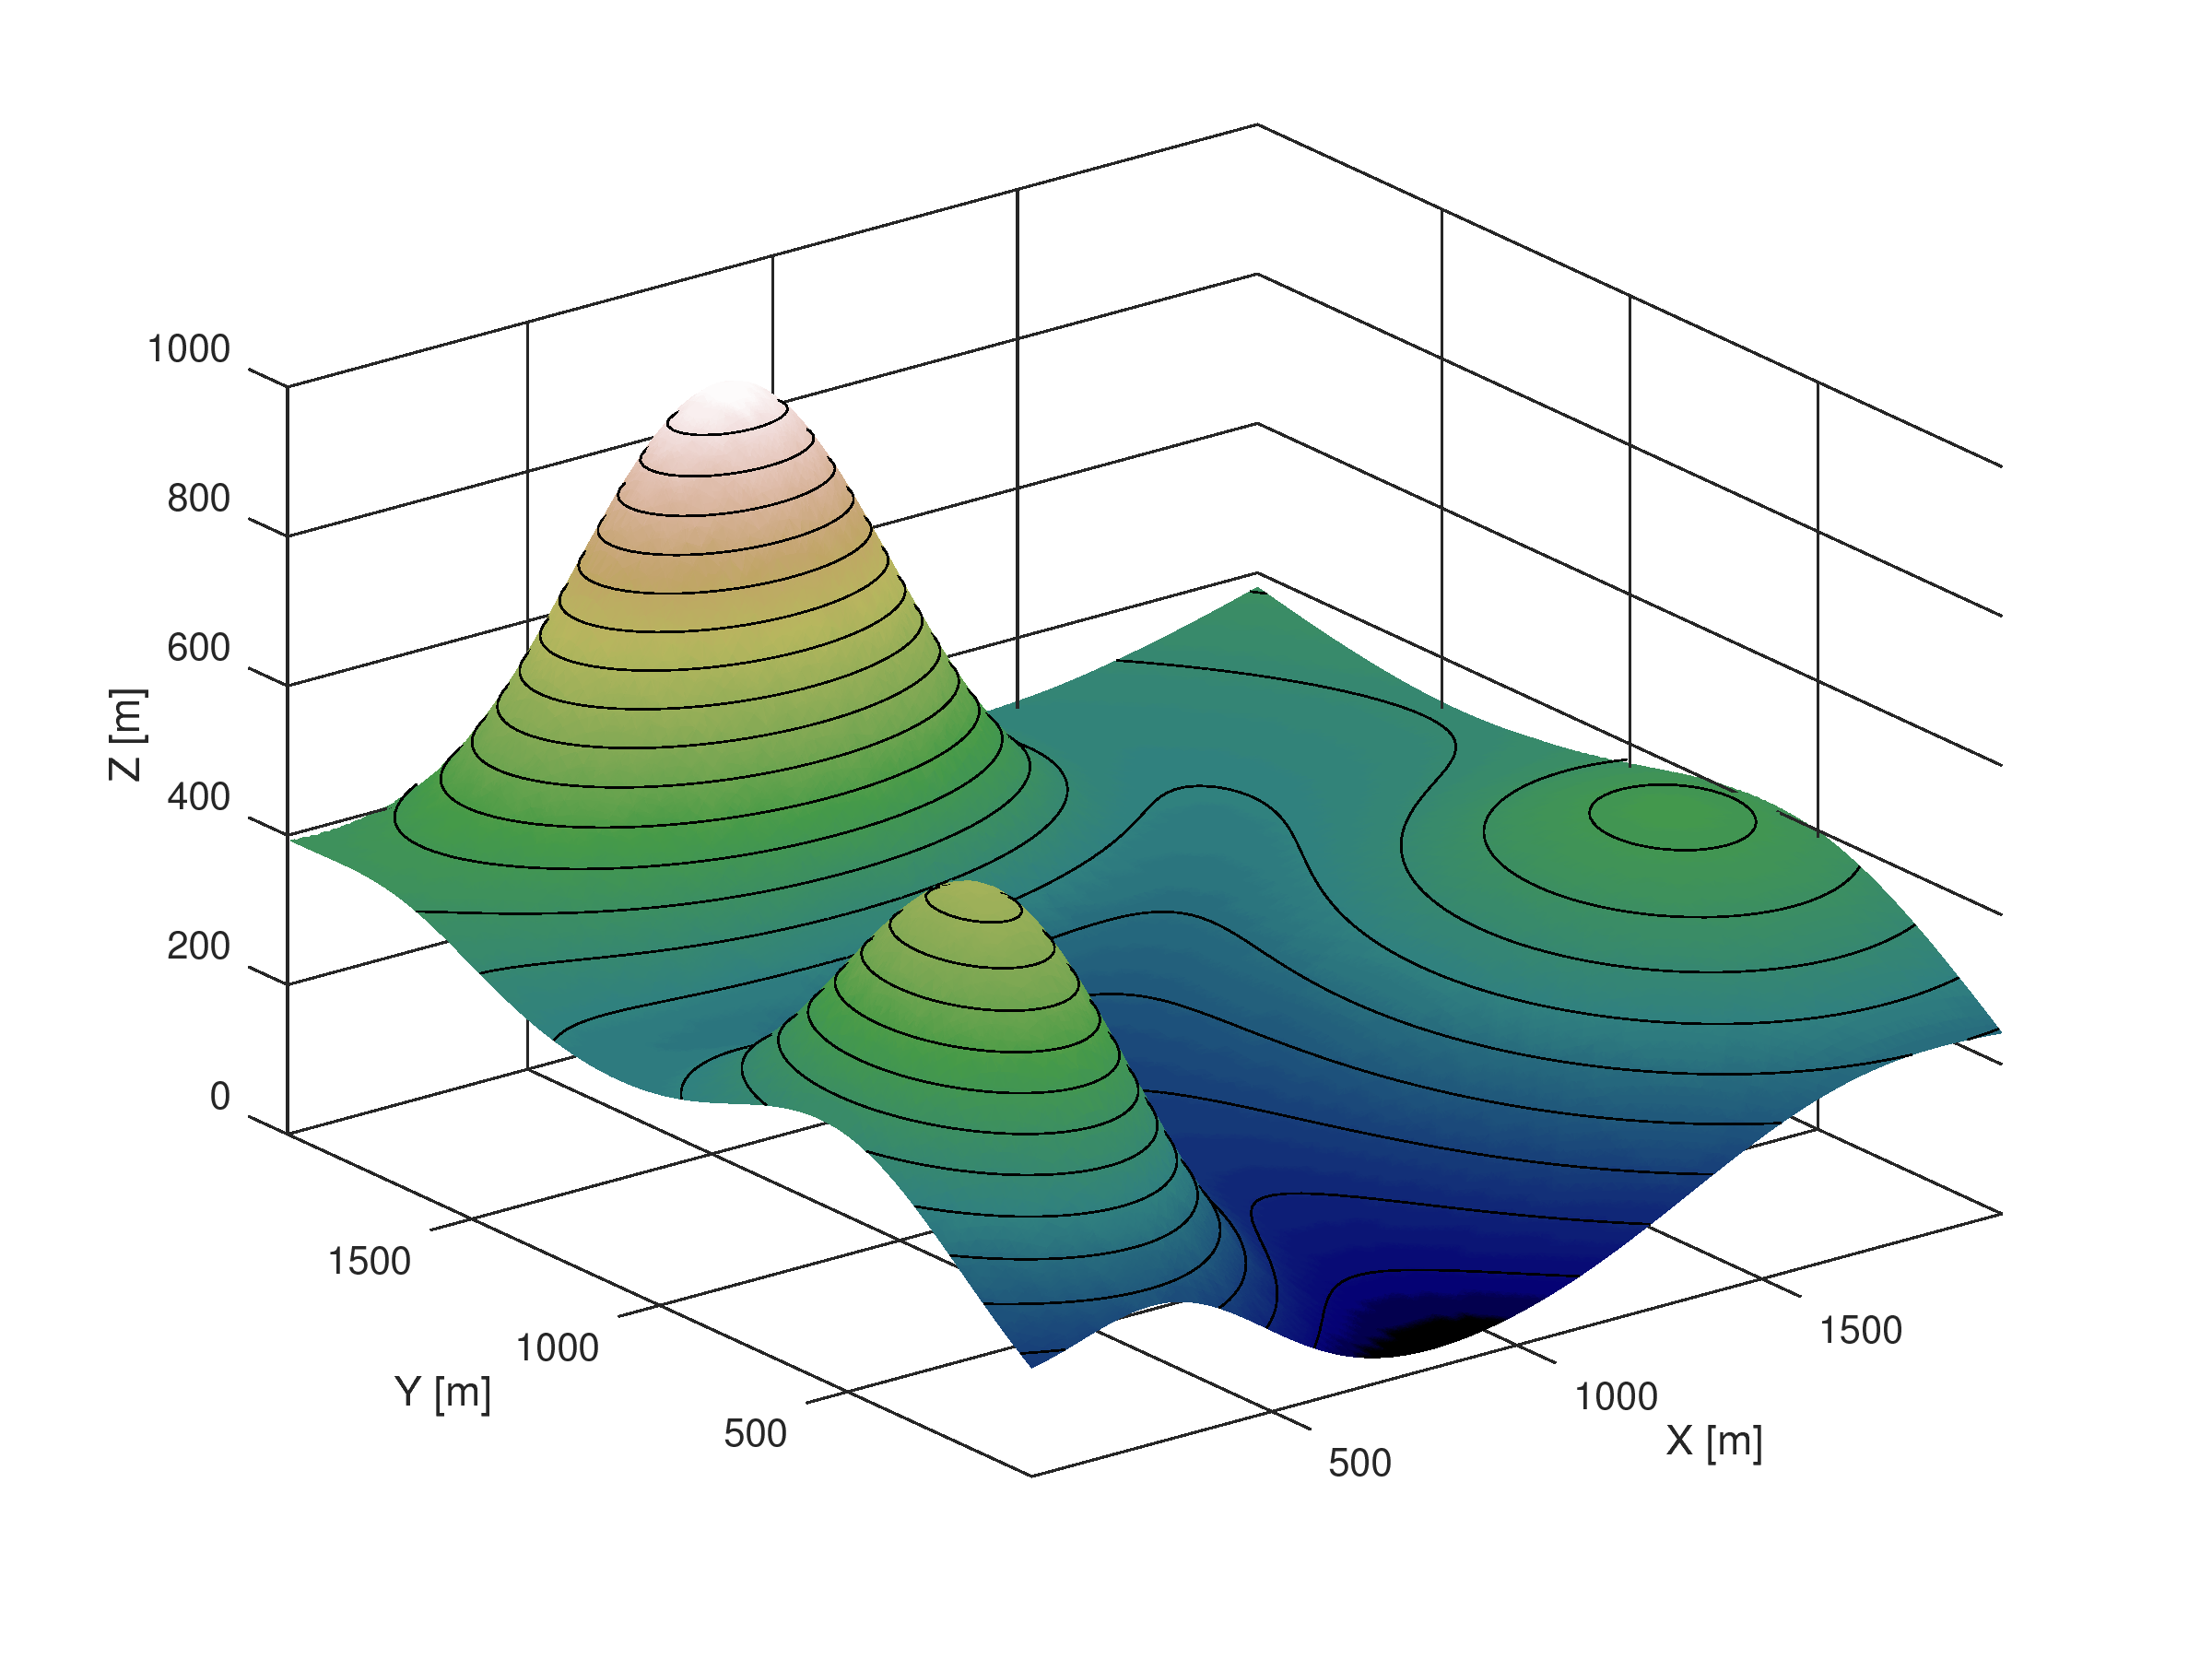
\includegraphics[width=0.7\textwidth]{Figures/topography.png}
  \caption{Synthetic topography composed of three Gaussian bumps on a sloping plane.}
  \label{fig:topography}
\end{figure}

\begin{table}[htpb]
  \centering
  \caption{Parameters and setting fixed for all simulations.}
  \label{tab:simulations_parameters}
  \begin{threeparttable}
    \begin{tabular}{lrl}
      \toprule
      \textbf{Parameter} & \textbf{Value} & \textbf{Units} \\
      \midrule
      Domain x-length                          &    $2'000$           & \si{\meter}   \\
      Domain y-length                          &    $2'000$           & \si{\meter}   \\
      Number of cells x                        &    $100$             & --   \\
      Number of cells y                        &    $100$             & --   \\
      Friction coefficient\tnote{*}            &    $0.03$            & \si{s.m^{-1/3}}\\
      Crust thickness\tnote{*}                 &    $1$               & \si{\meter}\\
      Crust hydraulic conductivity\tnote{*}    &    $2\cdot 10^{-6}$  & \si{\meter\per\second}\\
      Soil hydraulic conductivity\tnote{*}     &    $2\cdot 10^{-6}$  & \si{\meter\per\second}\\
      Soil suction head\tnote{*}               &    $0.09$      & \si{\meter}\\
      Soil maximum infiltration rate\tnote{*}  &    $19.8$      & \si{\milli\meter\per\hour}\\
      \bottomrule
    \end{tabular}
    \begin{tablenotes}
      \item[*] Parameters spatially distributed.
    \end{tablenotes}
  \end{threeparttable}
\end{table}


% ===================================================================================================
\section{Generating the datasets}
% ===================================================================================================

The dataset required for building the emulator was generated by running \num{50} simulations with different combinations of the variables \emph{rain intensity} ($I$) and \emph{initial soil saturation} ($\theta_i$).
The initial soil saturation, being a spatially distributed variable, was kept uniform over the whole domain.
The rain intensity was also uniformly applied over the domain, also since \textit{FullSWOF\_2D}, at this stage of development, only allows for uniformly distributed rain events.
\num{5} different initial saturations in the $[\numrange{0}{1}]$ interval and \num{10} rain intensities in the \SIrange{10}{35}{\milli\metre\per\hour} interval were taken and all their possible combinations were used as inputs for the simulations.
This data constitute the \emph{training dataset} for the emulator.
A \emph{test dataset} and a \emph{validation dataset} were also generated.
These datasets can be found in the Appendix~\ref{AppendixB}.

Some parameters, namely those specific for the catchment in questions, were kept constant over all of the simulations.
This are summarized in Tab.~\ref{tab:simulations_parameters}.
The parameters marked with * are those \emph{spatially distributed}, meaning that a different value could be set for every cell.
For simplicity, a spatially uniform catchment was used, therefore the values from the table are valid for the whole domain.


\begin{figure}[htpb]
  \centering
  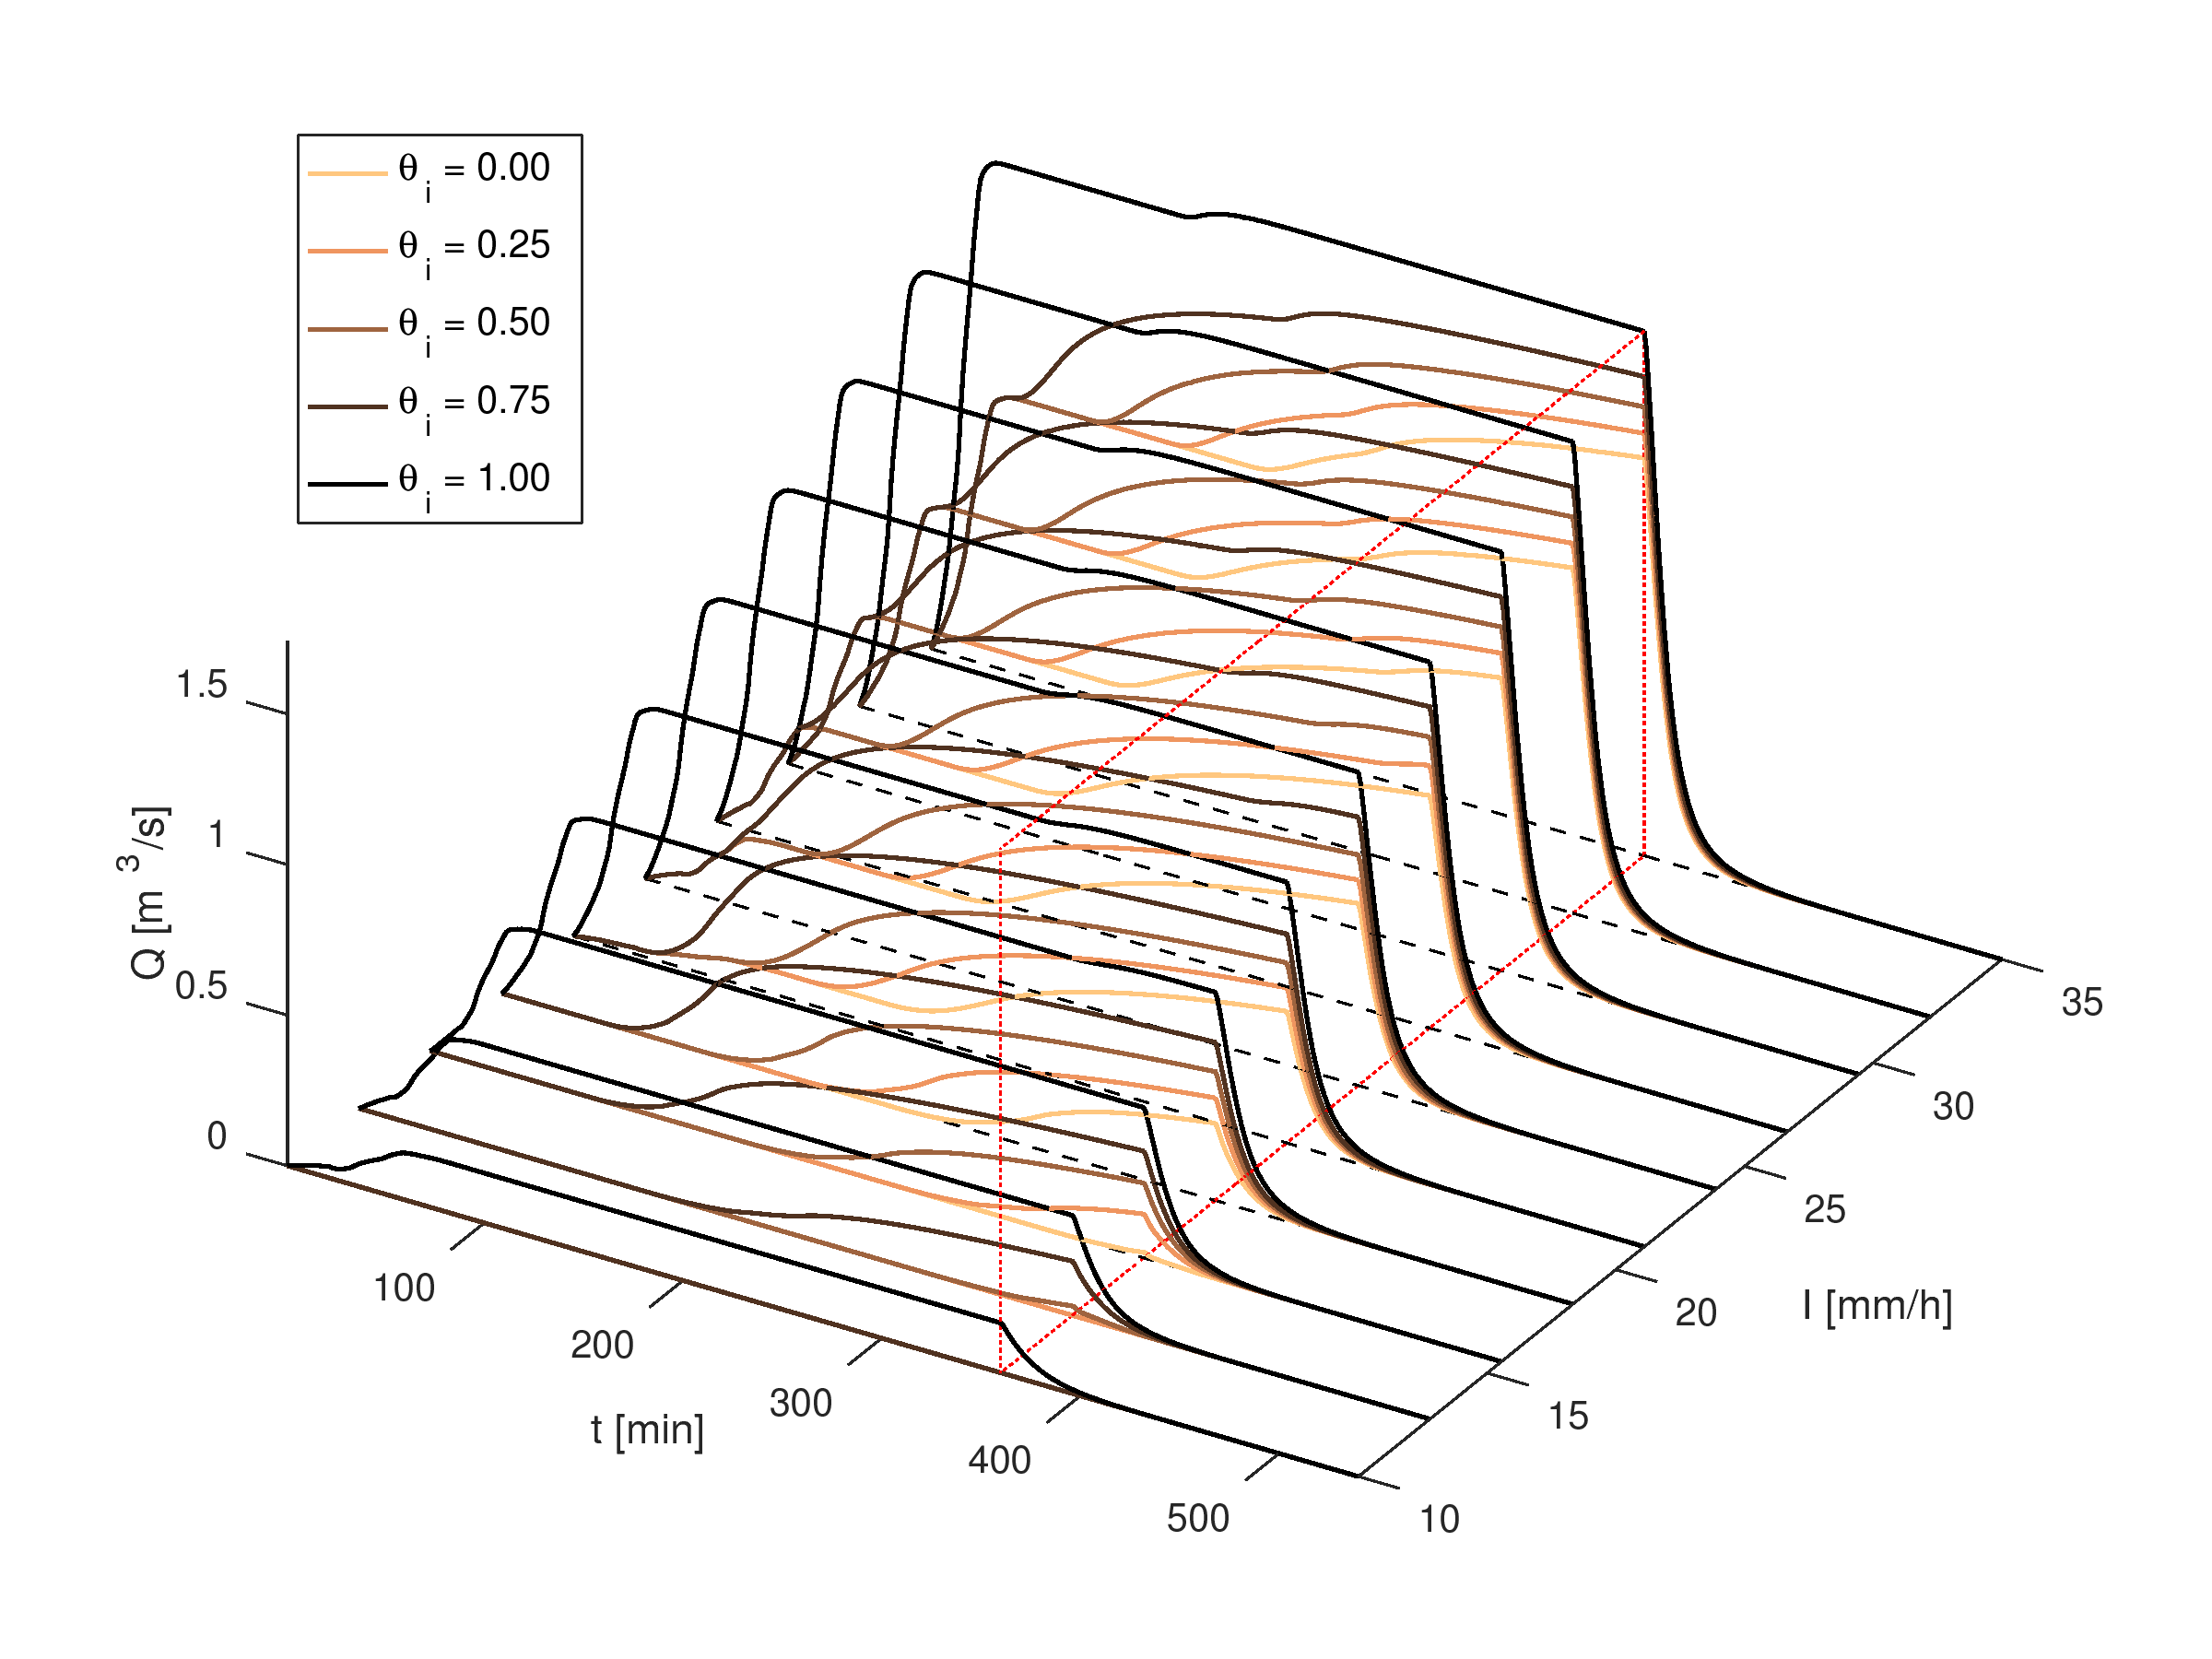
\includegraphics[width=0.75\textwidth]{Figures/hydrographs3d.png}
  \caption{Response hydrographs of the \num{50} simulations at the catchment outlet.}
  \label{fig:hydrographs3d}
\end{figure}


% ===================================================================================================
\section{Building the emulator}
% ===================================================================================================

% ---------------------------------------------------------------------------------------------------
\subsection{Classification emulator}
% ---------------------------------------------------------------------------------------------------

% ---------------------------------------------------------------------------------------------------
\subsection{Time-to-threshold emulator}
% ---------------------------------------------------------------------------------------------------


